\section*{Results}
\label{Results}
%Visualize and analyze your data with an appropriate hypothesis test and document the experiment.
%
Der blev i alt kørt otte testpersoner gennem testen. Testpersonerne brugt til undersøgelsen er studerende på Aalborg Universitet, herunder studieretningerne jura, kemi-teknologi, fysik og biologi. Testpersonernes alder strækker sig fra 21 år til 34 år med en gennemsnitsalder på 24,6 år.

\noindent En præsentation af de afgivne vurderinger fra testpersonerne, inddelt efter personer, kan ses på \autoref{fig:RaaDataTestpersoner}. 

\begin{figure}[H]
\centering
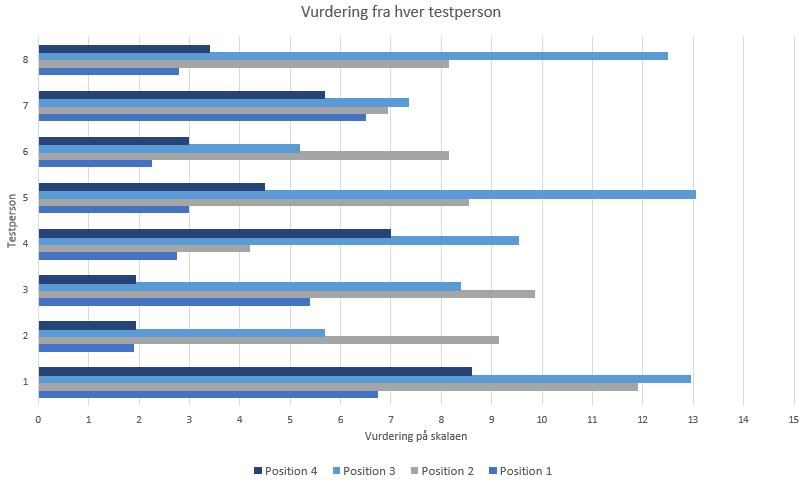
\includegraphics[width = \textwidth]{Figure/RaaDataTestpersoner.PNG} 
\caption{Rå data inddelt efter testpersoner}
\label{fig:RaaDataTestpersoner}
\end{figure}
%
\noindent På \autoref{fig:RaaDataPositioner} er vurderingerne præsenteret, hvor de er inddelt efter de fire positioner. Det giver et indblik i om en eller flere positioner kan være vurderet højere end andre. 
%
\begin{figure}[H]
\centering
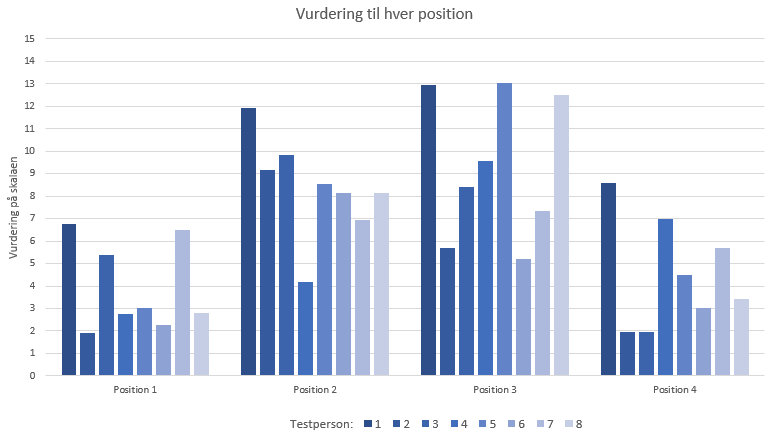
\includegraphics[width = \textwidth]{Figure/RaaDataPositioner.PNG} 
\caption{Rå data inddelt efter de fire positioner}
\label{fig:RaaDataPositioner}
\end{figure}
%
\noindent For at kunne konkludere om der er en signifikant forskel mellem vurderingerne ved de forskellige positioner vælges det at lave en statistisk analyse. 